\SourceLeaf{319}
\subsection*{Transformations of the form $\left(\begin{smallmatrix}5,&5,&5\\-1,&-1,&-1\end{smallmatrix}\right)$ Det. $=108$}
\pdfbookmark[1]{Transformations of the form}{ternary-transformationen}
\begin{center}\scriptsize
\setlength{\tabcolsep}{2pt}
\begin{tabular}{ccccc l}
&&&&&Chaux carbonatée\\
$\left\{\begin{smallmatrix}+1&+1&-1\\-1&+1&+1\\+1&-1&+1\end{smallmatrix}\right\}$&
$\begin{gathered}\left(\begin{smallmatrix}17&17&17\\-7&-7&-7\end{smallmatrix}\right)\\36\pdot108\end{gathered}$&&
$\begin{gathered}\left(\begin{smallmatrix}240&240&240\\+168&+168&+168\end{smallmatrix}\right)\\256\pdot11664\end{gathered}$&
$\begin{gathered}\left(\begin{smallmatrix}10&10&10\\+7&+7&+7\end{smallmatrix}\right)\\216\end{gathered}$&equiaxe\\[1.4ex]
$\left\{\begin{smallmatrix}+1&+1&0\\0&+1&+1\\+1&0&+1\end{smallmatrix}\right\}$&
$\begin{gathered}\left(\begin{smallmatrix}8&8&8\\+2&+2&+2\end{smallmatrix}\right)\\4\pdot108\end{gathered}$&
$\begin{gathered}\left(\begin{smallmatrix}4&4&4\\+1&+1&+1\end{smallmatrix}\right)\\54\end{gathered}$&
$\begin{gathered}\left(\begin{smallmatrix}15&15&15\\-3&-3&-3\end{smallmatrix}\right)\\27\pdot108\end{gathered}$&
$\begin{gathered}\left(\begin{smallmatrix}5&5&5\\-1&-1&-1\end{smallmatrix}\right)\\54\end{gathered}$&inverse\\[1.4ex]
$\left\{\begin{smallmatrix}+2&+1&+1\\+1&+2&+1\\+1&+1&+2\end{smallmatrix}\right\}$&
$\begin{gathered}\left(\begin{smallmatrix}20&20&20\\+14&+14&+14\end{smallmatrix}\right)\\16\pdot108\end{gathered}$&
$\begin{gathered}\left(\begin{smallmatrix}10&10&10\\+7&+7&+7\end{smallmatrix}\right)\\216\end{gathered}$&
$\begin{gathered}\left(\begin{smallmatrix}51&51&51\\-21&-21&-21\end{smallmatrix}\right)\\432\pdot108\end{gathered}$&
$\begin{gathered}\left(\begin{smallmatrix}17&17&17\\-7&-7&-7\end{smallmatrix}\right)\\16\pdot108\end{gathered}$&contrastante\\[1.4ex]
$\left\{\begin{smallmatrix}+1&+2&+2\\+2&+1&+2\\+2&+2&+1\end{smallmatrix}\right\}$&
$\begin{gathered}\left(\begin{smallmatrix}29&29&29\\+23&+23&+23\end{smallmatrix}\right)\\25\pdot108\end{gathered}$&&
$\begin{gathered}\left(\begin{smallmatrix}312&312&312\\-138&-138&-138\end{smallmatrix}\right)\\67500\pdot108\end{gathered}$&
$\begin{gathered}\left(\begin{smallmatrix}52&52&52\\-23&-23&-23\end{smallmatrix}\right)\\33750\end{gathered}$&mixte
\end{tabular}\end{center}

Writing the original form generally as $\left(\begin{smallmatrix}t,&t,&t\\u,&u,&u\end{smallmatrix}\right)$ and a derived form as $\left(\begin{smallmatrix}T,&T,&T\\U,&U,&U\end{smallmatrix}\right)$ gives
\[
\begin{array}{rll}
1,&T=3t-2u&U=-t+2u\\
2,&T=2t+2u&U=t+3u\\
3,&T=6t+10u&U=5t+11u\\
4,&T=9t+16u&U=8t+17u
\end{array}
\]

The form $\left(\begin{smallmatrix}1,&3,&k\\0,&0,&0\end{smallmatrix}\right)$ is transformed by the substitution
\[
\begin{array}{lll}
x=u+u'-2u''&\text{inversely}&6u=x+3y+2z\\
y=u-u'&&6u'=x-3y+2z\\
z=u+u'+u''&&6u''=-2x+2z
\end{array}
\]
\[
x\equiv z'\pmod3,\quad x\equiv y\pmod2
\]
into $\left(\begin{smallmatrix}4+k,&4+k,&4+k\\k-2,&k-2,&k-2\end{smallmatrix}\right)$

To obtain calcite, set $k=0{,}973103$.

Hind the complex values of the orthographic projection of three straight lines of equal length and perpendicular to one another be $a,b,c$, then $aa+bb+cc=0$; in general, with $p$ and $q$ denoting arbitrary complex numbers, one may set
\[
\begin{gathered}
a=(p-q)(q-pii),\quad b=(q-qi)(pii-pi),\\c=(qi-p)(pi-q)
\end{gathered}
\]

\clearpage
\SourceLeaf{320}
\subsection*{Hexakisoctahedron.}
\pdfbookmark[1]{Hexakisoctahedron}{ternary-hexakisoctaeder}
\begin{center}
\resizebox{!}{14mm}{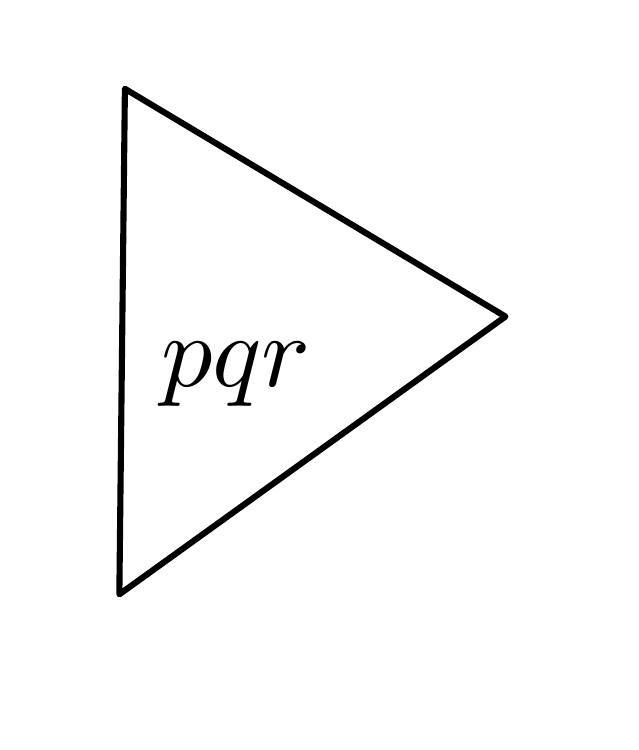
\begin{tikzpicture}[x=1bp,y=-1bp,line cap=round,line join=round]
\path[use as bounding box] (0,0) rectangle (210,250);
\begin{pgfinterruptboundingbox}
\draw[line width=2.2bp] (35,22) -- (172,104) -- (33,204) -- cycle;
\node[inner sep=0pt,outer sep=0pt,anchor=center] at (75,125) {\scalebox{3.7}{\ensuremath{pqr}}};
\end{pgfinterruptboundingbox}
\end{tikzpicture}
}\qquad Equation: $px+qy+rz=1$
\end{center}

\begin{center}\emph{Coordinates.}\end{center}
\begin{center}
\begin{minipage}{.28\textwidth}\centering
\resizebox{\linewidth}{!}{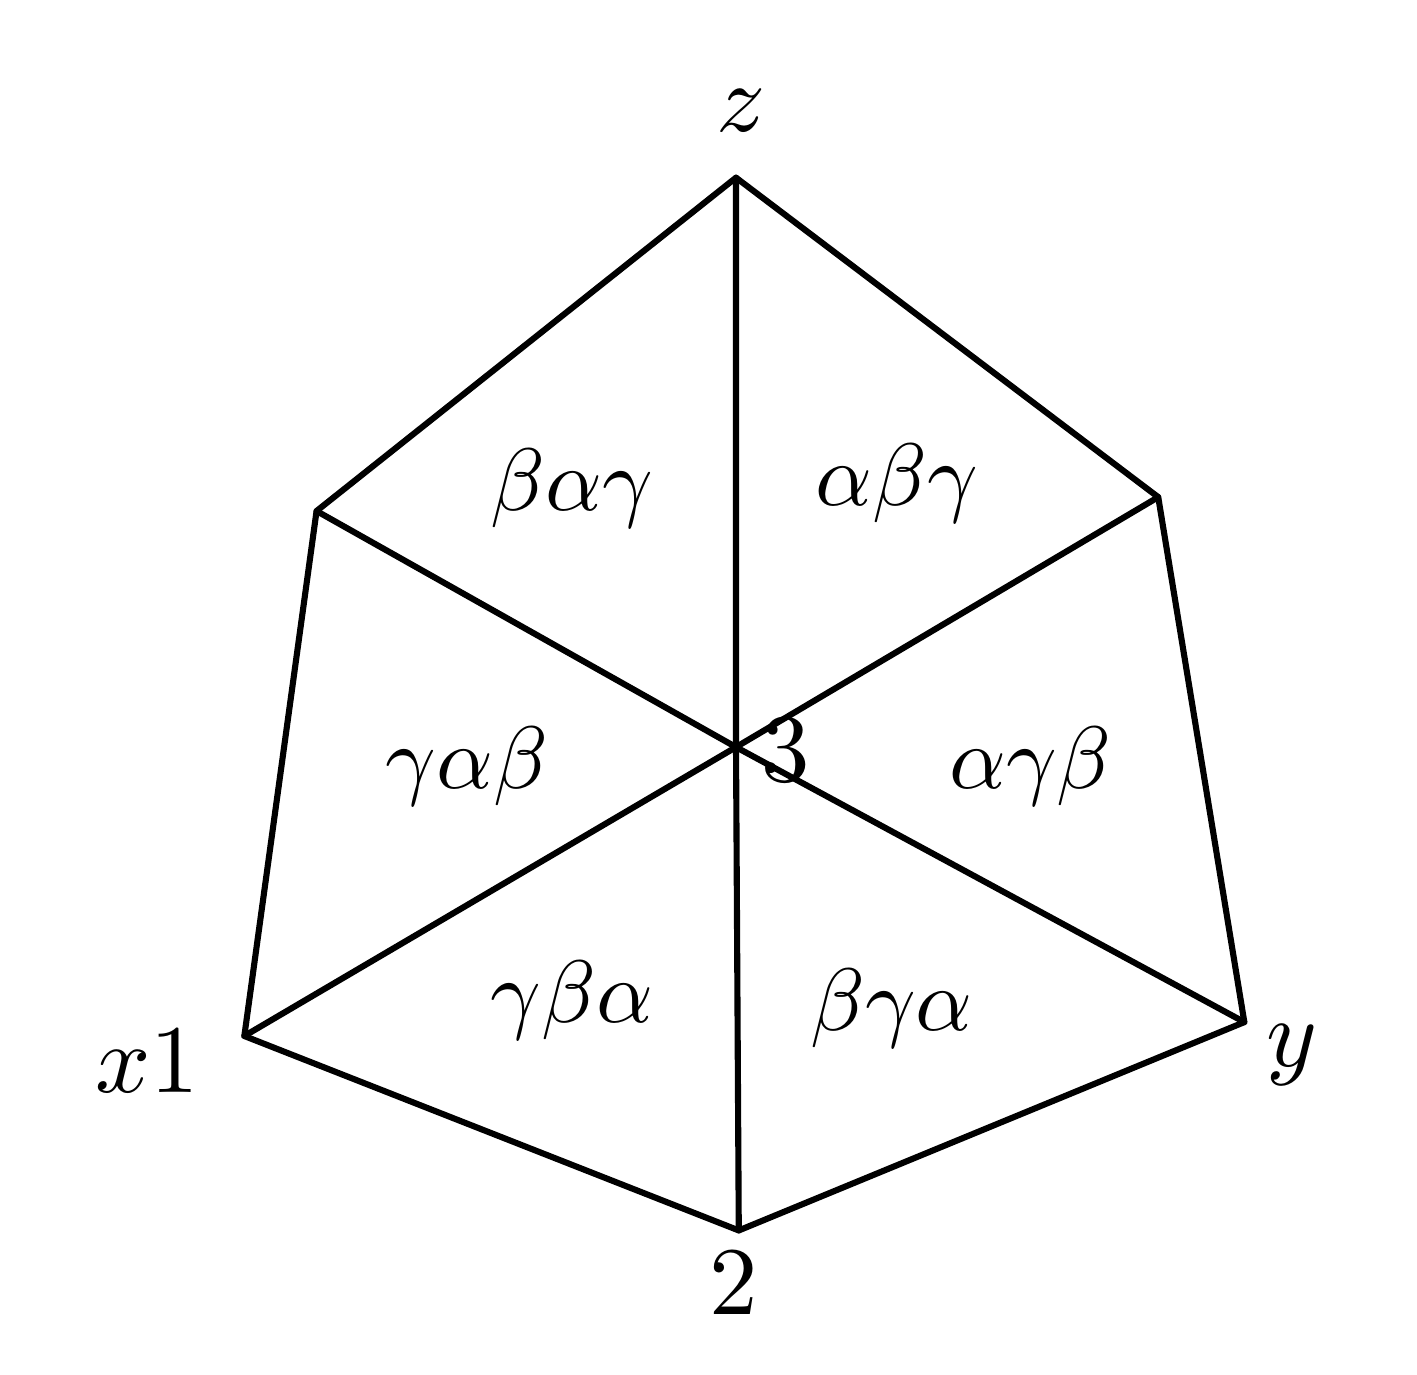
\begin{tikzpicture}[x=1bp,y=-1bp,line cap=round,line join=round]
\path[use as bounding box] (0,0) rectangle (490,475);
\begin{pgfinterruptboundingbox}
\draw[line width=2.2bp] (255,54) -- (407,169) -- (438,358) -- (256,433) -- (78,363) -- (104,174) -- cycle;
\draw[line width=2.2bp] (255,54) -- (255,259) -- (256,433);
\draw[line width=2.2bp] (104,174) -- (255,259) -- (438,358);
\draw[line width=2.2bp] (78,363) -- (255,259) -- (407,169);
\node[inner sep=0pt,outer sep=0pt,anchor=center] at (196,166) {\scalebox{3.2}{\ensuremath{\beta\alpha\gamma}}};
\node[inner sep=0pt,outer sep=0pt,anchor=center] at (313,164) {\scalebox{3.2}{\ensuremath{\alpha\beta\gamma}}};
\node[inner sep=0pt,outer sep=0pt,anchor=center] at (158,266) {\scalebox{3.2}{\ensuremath{\gamma\alpha\beta}}};
\node[inner sep=0pt,outer sep=0pt,anchor=center] at (361,266) {\scalebox{3.2}{\ensuremath{\alpha\gamma\beta}}};
\node[inner sep=0pt,outer sep=0pt,anchor=center] at (196,350) {\scalebox{3.2}{\ensuremath{\gamma\beta\alpha}}};
\node[inner sep=0pt,outer sep=0pt,anchor=center] at (311,353) {\scalebox{3.2}{\ensuremath{\beta\gamma\alpha}}};
\node[inner sep=0pt,outer sep=0pt,anchor=center] at (257,30) {\scalebox{3.5}{\ensuremath{z}}};
\node[inner sep=0pt,outer sep=0pt,anchor=center] at (43,372) {\scalebox{3.5}{\ensuremath{x1}}};
\node[inner sep=0pt,outer sep=0pt,anchor=center] at (455,370) {\scalebox{3.5}{\ensuremath{y}}};
\node[inner sep=0pt,outer sep=0pt,anchor=center] at (254,452) {\scalebox{3.5}{\ensuremath{2}}};
\node[inner sep=0pt,outer sep=0pt,anchor=center] at (273,260) {\scalebox{3.5}{\ensuremath{3}}};
\end{pgfinterruptboundingbox}
\end{tikzpicture}
}
\[\alpha<\beta<\gamma\]
\end{minipage}\hfill
\begin{minipage}{.68\textwidth}
\[
\begin{array}{rccc}
1.&\dfrac1\gamma&0&0\\[1ex]
2.&\dfrac1{\beta+\gamma}&\dfrac1{\beta+\gamma}&0\\[1ex]
3.&\dfrac1{\alpha+\beta+\gamma}&\dfrac1{\alpha+\beta+\gamma}&\dfrac1{\alpha+\beta+\gamma}
\end{array}
\]
\end{minipage}
\end{center}

Six times the volume of an elementary pyramid
\[
=\frac1{\gamma\pdot(\beta+\gamma)(\alpha+\beta+\gamma)}
\]
All [faces] are circumscribed about a sphere whose radius
\[
=\frac1{\surd(\alpha\alpha+\beta\beta+\gamma\gamma)}
\]
Twice the area of a triangle
\[
=\frac{\surd(\alpha\alpha+\beta\beta+\gamma\gamma)}{\gamma(\beta+\gamma)(\alpha+\beta+\gamma)}
\]
Edge
\[
\begin{aligned}
1\pdot2&=\frac{\surd(\beta\beta+\gamma\gamma)}{\gamma(\beta+\gamma)},\\
1\pdot3&=\frac{\surd((\alpha+\beta)^2+2\gamma\gamma)}{\gamma(\alpha+\beta+\gamma)},\\
2\pdot3&=\frac{\surd(2\alpha\alpha+(\beta+\gamma)^2)}{(\beta+\gamma)(\alpha+\beta+\gamma)}
\end{aligned}
\]
Cosine of the angle between the edges $3\pdot1\pdot2$
\[
=\frac{\alpha\beta+\beta\beta+\gamma\gamma}{\surd(\beta\beta+\gamma\gamma)((\alpha+\beta)^3+2\gamma\gamma)}
\]
Sine
\[
=\frac{\gamma\pdot\surd(\alpha\alpha+\beta\beta+\gamma\gamma)}{\surd(\beta\beta+\gamma\gamma)((\alpha+\beta)^2+2\gamma\gamma)}
\]

\Needspace{23\baselineskip}
\begin{center}\emph{Values occurring.}\end{center}
\begin{center}
\begin{tabular}{rccc l}
&$\alpha$&$\beta$&$\gamma$&\\
7.&0.&0.&1&Hexahedron\\
3.&0.&1.&1&Rhombic dodecahedron\\
6.&0.&1.&2&Tetrakishexahedron\\
&0.&1.&3&\\
&0.&2.&3&\\
1.&1.&1.&1&Octahedron\\
5.&1.&1.&2&Deltoidal icositetrahedron\\
&1.&1.&3&\\[1.2ex]
&$\alpha$&$\beta$&$\gamma$&\\
2.&1.&2.&2.&Triakisoctahedron\\
4.&1.&2.&3.&Hexakisoctahedron\\
&1.&2.&4.&\\
2.&1.&3.&3.&Triakisoctahedron\\
4.&1.&3.&5.&Hexakisoctahedron\\
2.&2.&3.&3&Triakisoctahedron\\
&2.&3.&4?&\\
&3.&5.&11&
\end{tabular}
\end{center}
\BookRule{.36\textwidth}
